\section{Theoretische Grundlagen}
Der Compton-Effekt beschreibt die Vergrößerung der Wellenlänge von $\gamma$-Strahlung bei Streuung an einem Teilchen. Zur Untersuchung
des Compton-Effekts wird in diesem Versuch Röntgenstrahlung verwendet, da dieser Effekt nur bei hinreichend großen Energien festgestellt wird.
Bei Streuung der $\gamma$-Strahlung, beispielsweise an einem Plexiglasquader, lässt sich das Transmissionsverhalten analysieren. Dabei
sind zwei verschiedene Streuungsvorgänge zu erkennen, eine klassische inelastische Streuung und eine frequenzverschobene elastische Streuung.
\\
Die inelastische Streeung ist auch als Compton-Streuung bekannt. Das Photon gibt einen Teil seiner Energie an ein naheliegendes freies Elektron ab, ändert seine Wellenlänge und wird unter einem 
bestimmten Winkel $\theta$ gestreut. Das Elektron nimmt diese Energie in Form von kinetischer Energie auf. Aus der Energie- und Impulserhaltung kann die Wellenlängenanderung des Photons ermittelt werden.
Der Wellenlängenunterschied
\begin{equation*}
\increment \lambda = \lambda_{2} - \lambda_{1}
\end{equation*}
lässt sich durch die allgemeine Beschreibung der Photonenenergie
\begin{equation*}
E_{\text{ph}} = \frac{h \cdot c}{\lambda}
\end{equation*}
und einigen geometrischen Überlegungen als
\begin{equation}
\increment \lambda = \frac{h}{m_{e} c}(1-\text{cos}(\theta))
\end{equation}
angeben. Dabei ist $h$ das Plancksche Wirkungsquantum, $c$ die Lichtgeschwindigkeit und $m_{e}$ die Ruhemasse des Elektrons.
Der Proportionalitätsfaktor dieser Gleichung
\begin{equation}
\lambda_{c} = \frac{h}{m_{e} c}
\end{equation}
ist die sogenannte Compton-Wellenlänge die in diesem Versuch experimentell bestimmt werden soll. Der Streuwinkel liegt hierbei zwischen den
zwei Extremfällen. 
\begin{align*}
\theta = 0\textdegree \quad &\to \quad \increment \lambda = 0 \\
\theta = 180\textdegree \quad &\to \quad \increment \lambda = 2 \lambda_{c}
\end{align*}
Eine schematische Darstellung des Streuvorgangs ist in Abbildung \ref{fig:comptonstreuungskizze} dargestellt.
\begin{figure}
  \centering
  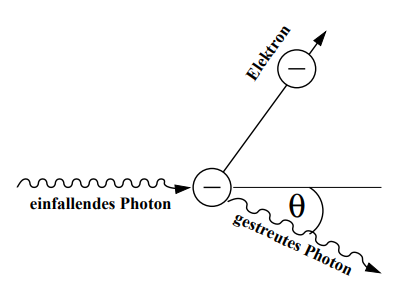
\includegraphics[width=0.5\textwidth]{bilder/comptonstreuung.png}
  \caption{Skizze des Streuvorgangs \cite{skript3}.}
  \label{fig:comptonstreuungskizze}
\end{figure}